\documentclass[useAMS, usenatbib, a4paper]{mnras}
\pdfsuppresswarningpagegroup=1

\usepackage{graphicx}
\usepackage{microtype}
\usepackage{xcolor}
\usepackage{fixltx2e}
\usepackage{booktabs}
\usepackage{siunitx}
\sisetup{separate-uncertainty = true}
\usepackage{color}
\usepackage{enumerate}
\usepackage{pdflscape}
\usepackage{rotating}
\usepackage{xr-hyper}
\usepackage{hyperref}
\externaldocument[Q-]{quadrics-bowshock}

\usepackage[T1]{fontenc} 
\usepackage[utf8]{inputenc}

% Fonts 
\usepackage{newtxtext}
% Note: newtxmath must come AFTER newtxtext
\usepackage[varvw,smallerops]{newtxmath}

\usepackage{chemgreek}
\activatechemgreekmapping{newtx}

\hypersetup{colorlinks=True, linkcolor=blue!50!black, citecolor=black,
  urlcolor=blue!50!black}

\usepackage{etoolbox}
\robustify\bfseries
\robustify\itshape

%% The following hack solves a problem with
%% ERROR: \pdfendlink ended up in different nesting level than \pdfstartlink.
%% See https://tex.stackexchange.com/a/249743
\makeatletter
\patchcmd\@combinedblfloats{\box\@outputbox}{\unvbox\@outputbox}{}{%
  \errmessage{\noexpand\@combinedblfloats could not be patched}%
}%
\makeatother

%% Bold italic
\newcommand\hmmax{0}            % we don't need heavy fonts
\newcommand\bmmax{1}            % reduce use of math alphabets for bold
\usepackage{bm}

%% Bundled custom packages
\usepackage{aastex-compat}

\title
% {No radiation supported dust wave around \(\sigma\) Orionis}
% OR
{\boldmath A dusty bow shock around \(\sigma\) Orionis driven by an enclosed proplyd?}

\newcommand\AddressCRyA{Instituto de Radioastronom\'{\i}a y Astrof\'{\i}sica,
  Universidad Nacional Aut\'onoma de M\'exico, Apartado Postal 3-72,
  58090 Morelia, Michoac\'an, M\'exico}
\author[Henney \& Arthur]{
  William J. Henney \& S. Jane Arthur\\
  \AddressCRyA
}

% These dates will be filled out by the publisher
\date{Accepted XXX. Received YYY; in original form ZZZ}

% Enter the current year, for the copyright statements etc.
\pubyear{2017}
\DeclareMathOperator{\sgn}{sgn}
\DeclareMathOperator{\Sin}{\mathcal{S}}
\DeclareMathOperator{\Cos}{\mathcal{C}}
\DeclareMathOperator{\Cot}{\mathcal{T}}
\DeclareMathOperator{\GammaFunc}{\Gamma}
\newcommand\w{\ensuremath{\mathrm{w}}}
\newcommand\C{\ensuremath{\mathrm{c}}}
\providecommand{\abs}[1]{\lvert#1\rvert}
\providecommand{\Abs}[1]{\left\lvert#1\right\rvert}
\newcommand\TODO[1]{%
  \begin{center}
    \framebox{\parbox{0.8\linewidth}{
        \texttt{\footnotesize\color{red} #1}}}
  \end{center}}

\newcommand\uvec[1]{\bm{\hat{#1}}}
\newcommand\T{_{\mathrm{\scriptscriptstyle T}}}

\newcommand\Qp{\ensuremath{Q_{\text{p}}}}
\newcommand{\grain}{\ensuremath{_{\text{d}}}}
\newcommand{\B}{\ensuremath{_{\scriptscriptstyle\text{B}}}}
\newcommand{\alfven}{\ensuremath{_{\scriptscriptstyle\text{A}}}}
\newcommand{\xsec}{\ensuremath{\sigma\grain}}
\newcommand\frad{\ensuremath{f_{\text{rad}}}}
\newcommand\fmax{\ensuremath{f_{\text{max}}}}
\newcommand\thm{\ensuremath{\theta_{\text{m}}}}
\newcommand\drag{\ensuremath{_{\text{drag}}}}
\newcommand{\gas}{\ensuremath{_{\text{gas}}}}
\newcommand{\drift}{\ensuremath{_{\text{drift}}}}
\newcommand\rad{\ensuremath{_{\text{rad}}}}
\newcommand\Rmin{\ensuremath{R_{\scriptscriptstyle\text{min}}}}
% Why do I need both of these?
\newcommand\sound{\ensuremath{c_{\text{s}}}}
\newcommand\soundspeed{\ensuremath{c_{\text{s,gas}}}}
\newcommand\starstar{\ensuremath{_{**}}}
\newcommand\hii{\ion{H}{ii}}


\defcitealias{Tarango-Yong:2018a}{Paper~I}
\newcommand\PaperI{\citetalias{Tarango-Yong:2018a}}


\begin{document}
\label{firstpage}
\pagerange{\pageref{firstpage}--\pageref{lastpage}}
\maketitle
\begin{abstract}
  We critically evaluate the role of radiation and hydrodynamics in
  providing internal support for the bow-shaped infrared arc around
  the massive triple star system \(\sigma\)~Ori Aa/Ab/B in the IC434 \hii{}
  region.  We present evidence for hydrogen recombination line
  emission from the arc, which demonstrates that it cannot be a
  decoupled dust wave, as has previously been claimed.  On the other
  hand, we show that the fraction of the stellar luminosity trapped by
  the arc is insufficient for it to be supported by radiation if the
  grains and gas are well coupled.  Therefore, the arc must be
  supported by the ram pressure of an internal wind.  However, the
  stellar winds from the OB stars in the \(\sigma\)~Ori Aa/Ab/B system seem
  too weak to provide this support on their own.  We propose instead
  that it is the photoevaporated disk wind from the enclosed proplyd
  IRS~1B that dominates the ram pressure support for the bow.
\end{abstract}

\begin{keywords}
  circumstellar matter -- radiation: dynamics -- stars: winds, outflows
\end{keywords}

\section{Why the inner arc cannot be a decoupled dust wave}
\label{sec:why-not-dust}

\section{Why the inner arc cannot be radiation-supported}
\label{sec:why-not-radiation}

SEDs of the two arcs

\begin{figure}
  \centering
  \includegraphics[width=\linewidth]{figs/sigma-ori-comparison}
  \caption{Optical and infrared images of $\sigma$~Ori}
  \label{fig:sig-ori}
\end{figure}

\begin{figure}
  \centering
  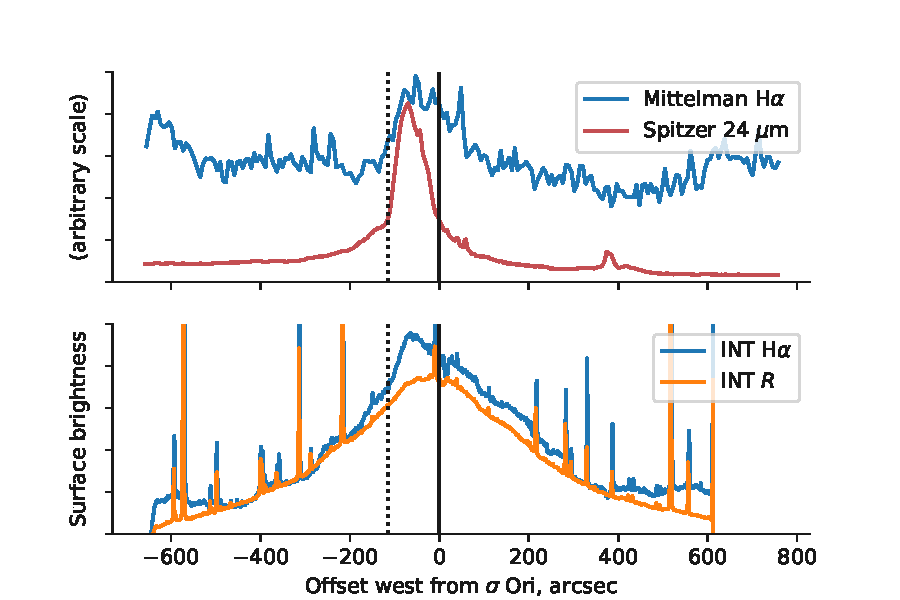
\includegraphics[width=\linewidth]{figs/sigma-ori-eastwest-cuts}
  \caption{Brightness profiles through $\sigma$~Ori inner arc.}
  \label{fig:sig-ori-cuts}
\end{figure}

\begin{figure}
  \centering
  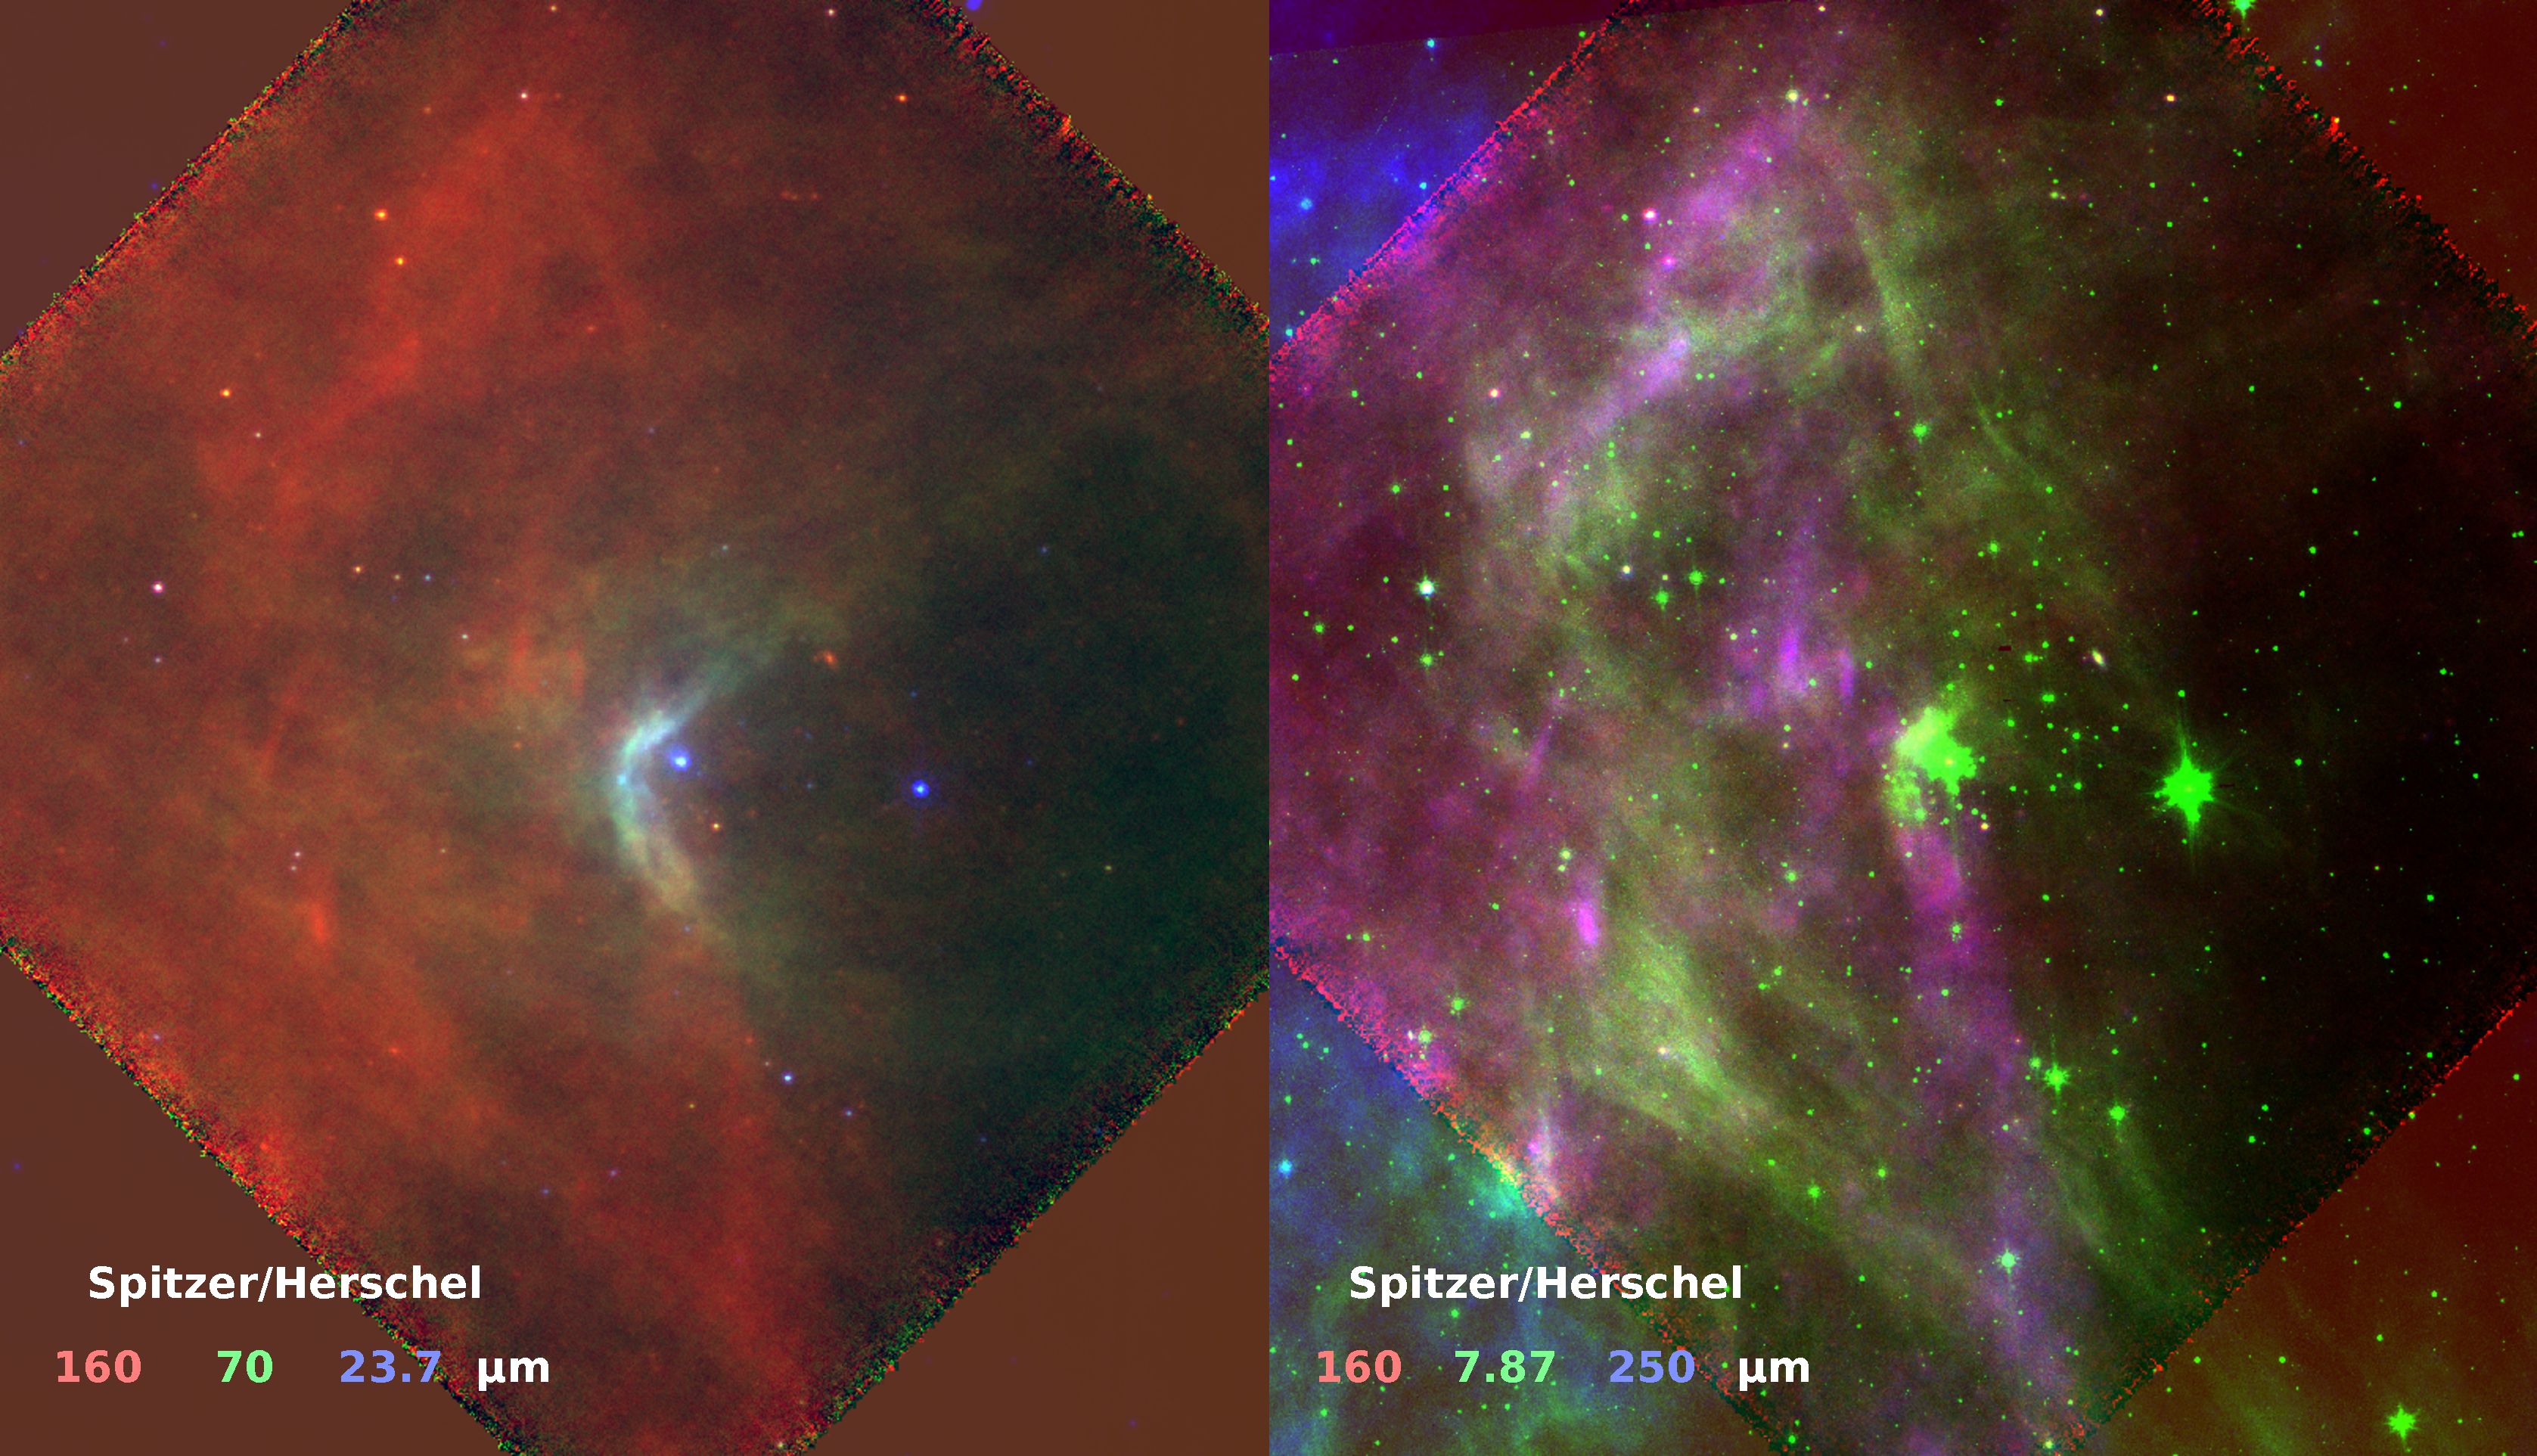
\includegraphics[width=\linewidth]{figs/sigma-ori-inner-outer}
  \caption{Combined mid-infrared and far-infrared views of the inner and outer arcs around $\sigma$~Ori}
  \label{fig:sig-ori-outer}
\end{figure}

\begin{figure}
  \centering
  \caption{Spectral energy distributions of arcs around $\sigma$~Ori}
  \label{fig:sig-ori-SED}
\end{figure}



\section{Weak stellar winds from the massive triple Aa/Ab/B}
\label{sec:stellar-winds-AB}

\section{Photoevaporation flow from the proplyd IRS~1B}
\label{sec:phot-flow-from}

\section{The nature of the outer dust arc}

\section{Conclusions}
\label{sec:conclusions}



\bibliographystyle{mnras}
\bibliography{bowshocks-biblio}

% Don't change these lines
\bsp	% typesetting comment
\label{lastpage}
\end{document}

%%% Local Variables:
%%% mode: latex
%%% TeX-master: t
%%% End:
